\documentclass[10pt,a4paper]{article}

\usepackage[margin=1.4cm,top=1.1cm,bottom=1.1cm]{geometry}
\usepackage{booktabs}
\usepackage{graphicx}
\usepackage{hyperref}
\usepackage{xcolor}
\usepackage{microtype}
\usepackage{tabularx}
\usepackage{enumitem}

\hypersetup{
    colorlinks=true,
    linkcolor=teal,
    urlcolor=blue,
    citecolor=teal
}

\pagestyle{empty} % Exactly one single-page note

\definecolor{codebg}{HTML}{F6F8FA}

\newcommand{\cmdbox}[1]{%
  \vspace{0.15em}%
  \noindent\colorbox{codebg}{%
    \parbox{\dimexpr\linewidth-2\fboxsep\relax}{\raggedright\ttfamily\small #1}%
  }%
  \vspace{0.15em}%
}

\begin{document}

\begin{center}
    {\LARGE \textbf{Technical Note: Snake Game Architecture \& Specifications}}\\[0.25em]
    {\normalsize \textbf{Author:} \texttt{mlr-agent-lab} \quad \textbullet \quad \textbf{Date:} October 14, 2026 \quad \textbullet \quad \textbf{Repository:} \href{https://github.com/kafcoo/mlr-agent-lab}{kafcoo/mlr-agent-lab}}
\end{center}

\vspace{-0.6em}
\noindent\rule{\textwidth}{0.5pt}
\vspace{-0.6em}

\subsection*{1. System Overview}
\vspace{-0.3em}
This technical note details the structural parameters, runtime mechanics, and automated verification harness of the retro Snake game implemented in pure HTML5 and Canvas 2D. The architecture decouples visual rendering from state updates using a fixed-frequency tick engine and a non-reversing input queue.

\vspace{-0.4em}
\subsection*{2. Visual Architecture \& Gameplay Capture}
\vspace{-0.3em}
\begin{figure}[h!]
    \centering
    % Sized prominently to maximize visual clarity while strictly maintaining 1-page budget
    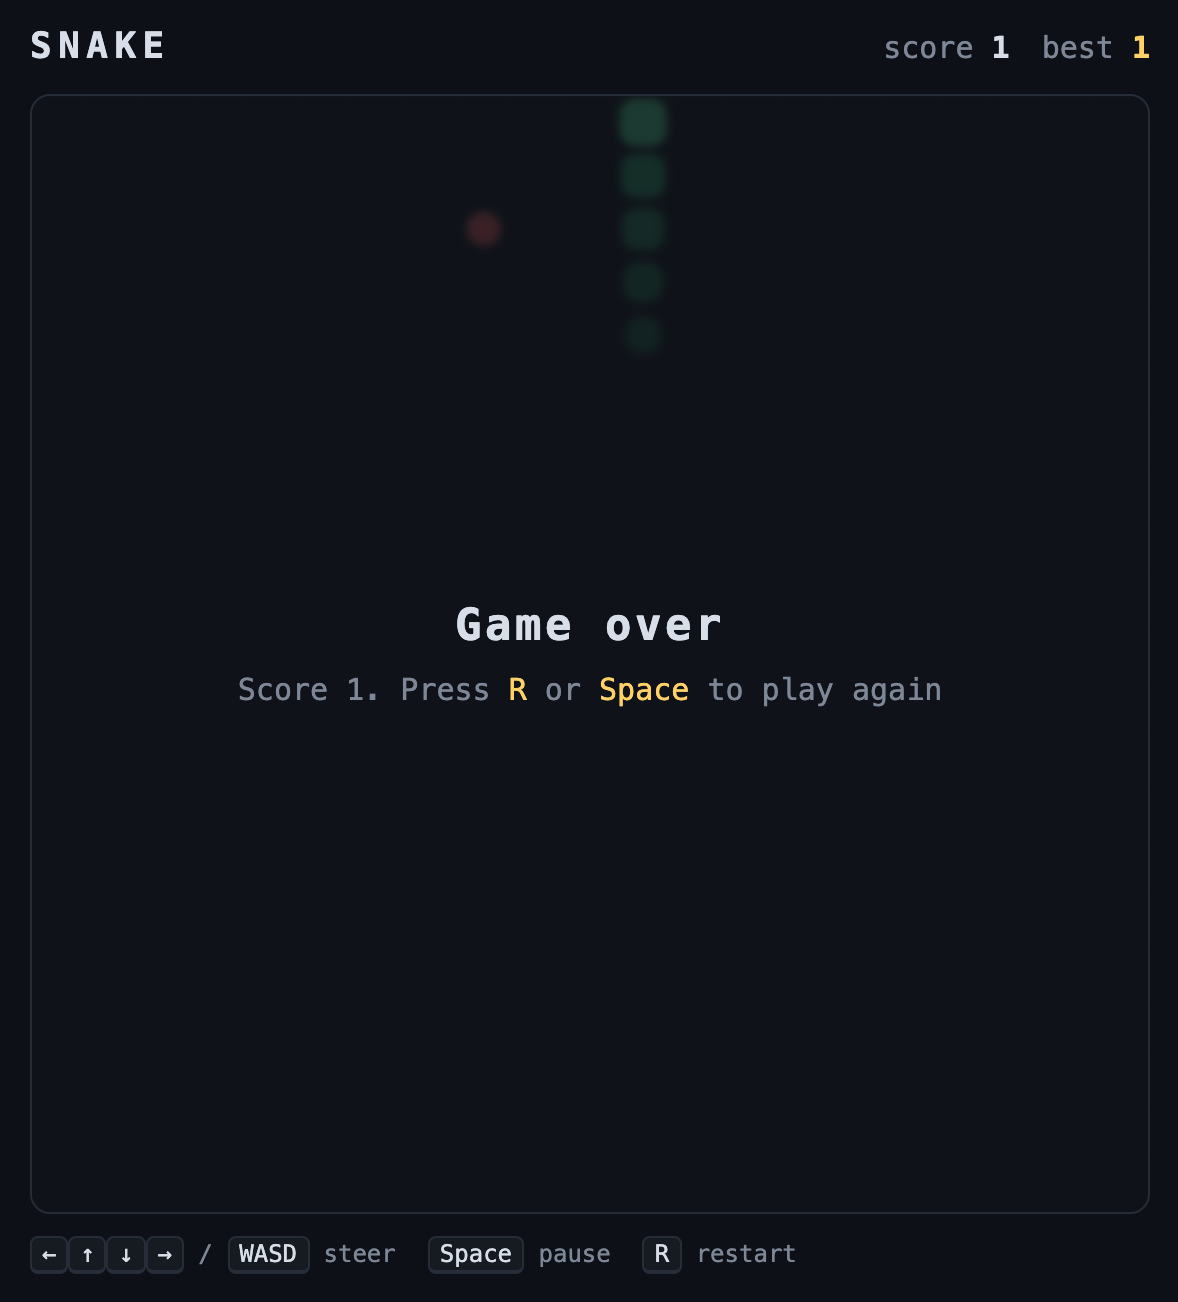
\includegraphics[width=0.55\textwidth,height=6.4cm,keepaspectratio]{assets/snake_screenshot_cropped.png}
    \vspace{-0.4em}
    \caption{Active gameplay state captured over Chrome DevTools Protocol (CDP) showing score HUD, arena border, snake body segments, overlay prompt, and controls.}
    \label{fig:gameplay}
\end{figure}

\vspace{-1.4em}
\subsection*{3. Dimensional Specifications \& Engine Constants}
\vspace{-0.3em}
\noindent
\begin{table}[h!]
    \centering
    \small
    \begin{tabularx}{\textwidth}{l p{3.2cm} X}
        \toprule
        \textbf{Parameter} & \textbf{Quantitative Value} & \textbf{Architectural Description \& Rationale} \\
        \midrule
        \textbf{Arena Grid} & $21 \times 21$ discrete cells & Odd-numbered dimensions allowing an exact symmetrical center origin. \\
        \textbf{Canvas Resolution} & $500 \times 500$ px & Coordinate raster scaled responsively via CSS \texttt{min(90vmin, 560px)}. \\
        \textbf{Unit Cell Pitch} & $23.8 \times 23.8$ px & Effective grid cell dimension on the rendering canvas. \\
        \textbf{Tick Interval} & $110$ ms ($9.09$ Hz) & Fixed simulation step balancing playability and collision responsiveness. \\
        \textbf{Initial Snake Length} & $4$ body segments & Starting configuration instantiated horizontally at row center $(y=10)$. \\
        \textbf{Input Turn Queue} & Depth: $3$ entries & FIFO buffer preventing key jamming and filtering out 180$^\circ$ self-reversals. \\
        \textbf{Food Entity} & $1$ unit cell ($20$ px) & Spawned in unallocated free cells using deterministic 32-bit PRNG. \\
        \bottomrule
    \end{tabularx}
\end{table}

\vspace{-1.3em}
\subsection*{4. Commands to Rebuild, Execute \& Test}
\vspace{-0.3em}
\begin{itemize}[leftmargin=*,itemsep=1.5pt,topsep=1pt]
    \item \textbf{Direct Interactive Viewer} (open in local browser):\\
    \cmdbox{open snake/index.html}
    \item \textbf{Rebuild Presentation Slides \& PDF Note}:\\
    \cmdbox{quarto render slides-with-animation-pdf-note/slides.qmd\\
    tectonic slides-with-animation-pdf-note/note.tex}
    \item \textbf{Automated Headless CDP Verification Test}:\\
    \cmdbox{uv run -{}-with websocket-client python /tmp/drive\_snake.py}
\end{itemize}

\vspace{-0.5em}
\subsection*{5. Project Links}
\vspace{-0.3em}
\begin{itemize}[leftmargin=*,itemsep=1pt,topsep=1pt]
    \item \textbf{Interactive Viewer}: \href{https://github.com/kafcoo/mlr-agent-lab/blob/main/snake/index.html}{\texttt{github.com/kafcoo/mlr-agent-lab/blob/main/snake/index.html}}
    \item \textbf{Automation Script}: \href{https://github.com/kafcoo/mlr-agent-lab}{\texttt{github.com/kafcoo/mlr-agent-lab (drive\_snake.py)}}
\end{itemize}

\end{document}
